\chapter{Entry Guidance for SRP-Based EDL}\label{Ch:FuelOptimalPaper}
%TODO: Examine this intro, merge some of it into the actual dissertation intro and leave the rest as the intro to this chapter...

Among the many considerable challenges involved in the Entry, Descent, and Landing (EDL) of a spacecraft on Mars, perhaps the greatest is the low density of the Martian atmosphere \cite{BraunMarsEDL, joel_dissertation}. At approximately one percent of the Earth's atmospheric density, current generation Mars entry vehicles are incapable of achieving sufficient deceleration to reach subsonic speeds before reaching the surface, necessitating the use of EDL technologies including supersonic parachutes and retropropulsion, both of which were utilized in safely landing MSL's Curiosity rover \cite{MSL_EDL}, and will also be utilized on the upcoming Mars 2020 mission \cite{M2020_EDL}. As the mass (or ballistic coefficient) of these vehicles grows, the problem is exacerbated until safe deployment conditions for current supersonic parachutes are not reachable at altitudes high enough to provide sufficient timeline margin for subsequent EDL events \cite{BraunMarsEDL}. In such missions, supersonic retropropulsion (SRP) may be relied upon to land larger, heavier vehicles relative to the current generation of landers without the use of a parachute, and as a result powered descent will play an even more significant role in the EDL process. In this paper, the emphasis is on the interplay between the entry phase and the powered phase, and thus only these two phases are considered.

%\textbf{It might be good to talk about the two phases here.}Figure~\ref{fig_phases} shows the two-phase EDL problem under consideration. 
The challenges during the entry phase from a guidance perspective include entry state dispersions due to delivery errors, atmospheric winds and density uncertainty, aerodynamic uncertainty, and imperfect onboard state estimation, each of which contribute to the size of the landing footprint. To date, MSL is the only Mars entry system to utilize hypersonic guidance to autonomously steer the spacecraft toward the target, which resulted in a landing footprint nearly an order of magnitude smaller than previous unguided ballistic entries \cite{BraunMarsEDL}. 
It is expected that a feature of SRP-based EDL is the requirement for pinpoint accuracy, defined as a sub-100 meter landing ellipse \cite{GNC_Pinpoint}. Assuming an entry guidance meets the basic requirement of delivering the vehicle to a state from which the powered guidance can achieve pinpoint landing, dispersed entry trajectories result in increased propellant requirements, rather than contribute to the landing ellipse. As a result, rather than judge an entry guidance algorithm by its landing ellipse, the propellant cost or propellant mass fraction (PMF) of the powered descent trajectory may now be considered a primary metric.

A fundamental difference of retropropulsion-based EDL from parachute-based EDL architectures, even those that utilize a vertical powered descent phase with potential for a divert maneuver beforehand, lies in the set of desirable states at the termination of the entry phase. In parachute-based EDL, the terminal entry state is constrained by safe parachute deployment conditions defined by upper and lower limits on Mach number and dynamic pressure. The constraints are often translated into constraints on altitude and velocity using a model of the Martian atmosphere. In summary, when a chute is involved, the target set for entry guidance is the parachute deployment box coupled with small downrange and crossrange errors, combined with a well-aligned heading, and no restriction on flight path angle. 

Traditionally, the primary objective of bank angle modulation during entry is range control with lateral control as a secondary objective, and guidance approaches could treat the two problems as decoupled. During the mission design phase, the downrange distance is chosen to be compatible with the parachute deployment conditions and other mission parameters such as the entry flight path angle. The target set in SRP-based EDL is in some sense much larger, but with more coupling between the state variables because, for a given powered descent guidance, the final entry state determines if pinpoint landing can be achieved, and if so, the propellant mass required. All six entry state variables contribute to the propellant cost; the optimal downrange distance and altitude at which to ignite depend on both the velocity magnitude and the flight path angle, while aligning the heading eliminates crosstrack flight during powered descent. 

% Altering the objective of entry guidance to shaping the trajectory for the benefit of the powered descent phase thus encourages a coupled approach. 
%For example, MSL utilized a range control phase and a heading alignment phase. Once the heading is aligned, the bank angle command will remain zero until the termination of the entry phase. Thus, unless heading alignment is initiated at the right time for zero bank angle to lead to the best termination condition, blah blah.

There exist many guidance solutions to the powered descent problem, often with a focus on propellant optimality. Classes of such algorithms include G-FOLD \cite{gfold,gfold_flighttests} and other convex optimization-based methods, polynomial-based approaches including the venerated Apollo lunar descent guidance \cite{apollo_lunar}, indirect optimal control methods \cite{PropellantOptimalAdaptiveTrigger}, and many others. 

Far less attention has been given to the role of entry guidance when followed directly by a powered descent phase, without an intermediate phase that makes use of a parachute or other decelerator. Reference~\cite{LuAdaptiveEDL} presents one approach to entry guidance in a chuteless EDL architecture. Reference~\cite{LuAdaptiveEDL} correctly identifies the potential for integrating the entry phase with the subsequent powered descent phase as an opportunity to reduce propellant consumption, and the vehicle bank angle is modulated to perform range control, utilizing a bank profile that is linear-in-energy with one free parameter. Lateral logic to determine bank reversals is applied separately after solving for the bank angle magnitude. Reference~\cite{EDL_AllProp} investigated an alternative EDL scheme in which aerodynamic control during entry is foregone in favor of hypersonic retropropulsion, essentially eliminating the entry phase. 

The proposed entry guidance for SRP-based EDL is designed to deliver the vehicle to a target set of states from which pinpoint landing can be achieved in the subsequent powered descent phase. Of the reachable states in the target set, entry guidance steers the vehicle to the one that will require the minimum propellant mass for pinpoint landing. For the simulation testing in this paper, the target set is computed by solving optimal control problems. 
%Details of this computation are presented later. This mapping is utilized in two distinct ways. At points along a given entry trajectory, the propellant cost can be computed in order to determine the best ignition condition for that trajectory. Additionally, the bank angle profile can be modified to intersect a portion of the feasible ignition set with sufficiently low propellant cost, using the mapping.  
%If the trajectory is poor, there may be not suitable ignition point, and the bank angle profile should be modified.
The possibility of computing the powered descent controllable set to be used as a target set for an entry guidance algorithm was suggested in Ref.~\cite{SRP_ControllableSets}, wherein a procedure based on convex optimization was designed to efficiently compute it is given.

MSL triggered its parachute deployment and descent sequence using a velocity trigger \cite{MSL_EDL2}, while Mars 2020 will utilize a range trigger \cite{M2020_EDL} to dramatically decrease the size of the landing ellipse \cite{TriggerComparison2020}. A component of our approach is an onboard determination of when to trigger powered descent initiation.  In essence, the role of such a trigger is to ensure the minimum propellant ignition point is found along any entry trajectory that has at least one feasible ignition state. The theoretical developments behind one such trigger were introduced in Ref.~\cite{PropellantOptimalAdaptiveTrigger}, while Ref.~\cite{LuAdaptiveEDL} demonstrated its benefits over triggering at a fixed state variable, such as downrange, velocity, or energy.
One potential weakness of the trigger in Ref.~\cite{PropellantOptimalAdaptiveTrigger} is that it assumes a propellant optimal powered descent guidance. In theory, future Mars missions, especially those transporting humans, may very well consider a guidance algorithm with a different objective, such as prioritizing safety or even passenger comfort, as the bang-bang nature of propellant optimal powered descent solutions may not be suitable, despite the importance of limiting propellant consumption. 

Despite presenting an approach in which a prediction of the terminal entry state is available and being used to modulate the vehicle bank angle, in Ref.~\cite{LuAdaptiveEDL} only the current vehicle state is checked for triggering the powered descent initiation. Our approach to the triggering mechanism differs in that we utilize the predicted trajectory. This allows us to query the mapping from the powered descent guidance algorithm at points along the predicted trajectory to generate propellant consumption predictions.  The benefit of doing so is two-fold. Firstly, the propellant optimal ignition point along an entry trajectory can be determined for any subsequent powered descent guidance, even one that is itself not propellant optimal. Secondly, by making explicit use of these predictions in the entry guidance algorithm, the two phases become linked by more than just the onboard triggering strategy, and superior propellant performance can be achieved. 

%Additionally, as mentioned above, our proposed entry guidance approach utilizes the powered descent guidance to be employed in the subsequent phase, in order to generate predicted propellant costs along a predicted trajectory. In this approach, the bank angle is actively modulated to reduce predicted propellant consumption rather than achieve a range objective, thereby allowing the entry guidance algorithm to suitably shape the trajectory in preparation for powered descent. It is this coordinated effort that allows the proposed entry guidance to produce superior results over traditional entry guidance methods. 

%We note that Reference Fully-Propulsive Mars Atmos Strategies for High-Mass Payload Missions looked at chuteless architectures but did not utilize lifting for control, and instead employed HYPERsonic retropulsion.
\section{Entry Guidance Problem}
The problem under investigation in this chapter considers a two-phase EDL sequence consisting of an entry phase and a powered descent phase. The dispersions in vehicle state arising from the approach phase are modeled as delivery errors at the beginning of the EDL sequence. In the entry phase, the vehicle is guided via bank angle modulation and the vehicle state is described in spherical coordinates, as described in Chapter~\ref{Ch:Models}. In the descent phase, the vehicle is guided via supersonic retropropulsion with the equations of motion given in Cartesian coordinates. The reason for the choice of two different coordinate systems is to be consistent with the literature on each respective topic.
\begin{figure}[h!]
	\centering
	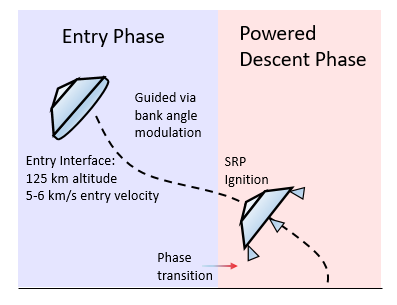
\includegraphics[width=0.5\textwidth]{../AAS20/EDLPhaseDiagram} 
	\caption{Schematic of the EDL phases}
	\label{fig_phases}
\end{figure}

Equations~\eqref{Eq:dynamics:radius:time}-\eqref{Eq:dynamics:heading:time} will be compactly referred to as $\dot{\mathbf{x}} = f(\mathbf{x},\sigma)$ and their solution at time $t$ from a state $\mathbf{x_0}$ evolving under a bank angle profile $\sigma[0,t]$ is given by the transition map $\mathbf{x}(t) = \varphi(t;\, \mathbf{x_0},\,\sigma[0,\,t])$.

%By solving the powered descent problem on the ground over a set of possible ignition states, an entry target set may be defined that allows us to reduce the two-phase problem to a problem with only an entry phase. In this new problem, the propellant required to land is only a function of the terminal entry state, because the powered descent thrust vector profile and time of flight are no longer optimization variables. Instead, the entire powered descent trajectory is now a function of the terminal entry state.  Hence, 
The entry guidance problem is to determine the entry phase duration and a bank angle profile that will deliver the vehicle from the entry interface to the propellant-optimal point in the target set, i.e., the set from which pinpoint landing can achieved. A formal definition of the target set is given in the subsequent section.
%\begin{align}
%\min \mathrm{prop}(\mathbf{x}(t_{pd})) \label{eq_entry_ocp}\\
%&\mathbf{x}(t_0) = \mathbf{x_0} \\
%&\mathbf{x}(t_{pd}) \in \mathcal{F}_M \\
%&\dot{\mathbf{x}} = f(\mathbf{x},\sigma)
%\end{align}

\subsection{Entry Guidance Target Set}
The entry guidance target set is defined by the powered descent algorithm to be used during the descent phase, and the available propellant onboard the vehicle. The equations of motion for a point mass vehicle in powered flight in a surface fixed frame, neglecting aerodynamic forces and Coriolis effects, are
\begin{align}
&\dot{\mathbf{r}} = \mathbf{v} \label{eq_eom_srp} \\
&\dot{\mathbf{v}} = \frac{\mathbf{T}}{m} + \mathbf{g}(\mathbf{r}) \\
&\dot{m} = -\frac{||\mathbf{T}||}{I_{sp}G_0} \label{eq_eom_srp_end}
\end{align}
where $\mathbf{r}\in\mathbb{R}^3$ is the position vector of the vehicle, $\mathbf{v}\in\mathbb{R}^3$ is the velocity vector of the vehicle, $m$ is its mass, $\mathbf{T}\in\mathbb{R}^3$ is the thrust vector of the vehicle, $\mathbf{g}\in\mathbb{R}^3$ is the gravitational acceleration vector, $I_{sp}$ is the specific impulse of the rocket engine, assumed to be constant, and $G_0$ is the gravitational acceleration magnitude at the surface of the Earth. The full powered descent state vector in $\mathbb{R}^7$ comprises the position, velocity, and mass. 

%The powered descent problem considered herein is to determine the optimal thrust magnitude and direction, as well the optimal time of flight, that solve the pinpoint landing boundary value problem comprising the equations of motion with prescribed initial and final conditions, while subject to constraints on the available thrust. 
Any powered descent algorithm capable of meeting the pinpoint landing requirement may be considered. To eschew the choice of a specific algorithm in this work, the powered descent problem is posed as the optimal control problem
\begin{align}
\max \;m(t_f) \label{eq_srp_ocp}\\
&\mathbf{r}(t_0) = \mathbf{r_0} \\
&\mathbf{v}(t_0) = \mathbf{v_0} \\
&m(t_0) = m_0\\
&\mathbf{r}(t_f) = [0,\, 0,\, z_{\mathrm{target}}] \\
&\mathbf{v}(t_f) = [0,\, 0,\, \dot{z}_{\mathrm{target}}] \\
0 <\,\, &T_{\min} \le ||\mathbf{T}(t)|| \le T_{\max}
\end{align}
%together with the dynamics Eq.~\ref{eq_eom_srp}-\ref{eq_eom_srp_end},
where the final time $t_f$ is free, $T_{\min}$ and $ T_{\max} $ are constant bounds on the available thrust, and $z_{\mathrm{target}}$ and $\dot{z}_{\mathrm{target}}$ are the desired altitude and vertical velocity at the end of the descent phase. For a fixed initial mass, maximizing the final mass is equivalent to minimizing the propellant use. Formulated as such, the optimal control problem can be viewed as a function $\mathrm{OCP}(\cdot)$ that maps an initial condition, i.e., ignition state, to a propellant cost. 
The set of initial states for which the optimal control problem has a feasible solution includes regions that are not of interest. Examples include states with initial altitudes very low to the ground, initial velocities much higher than those reachable by the entry vehicle before impacting the surface, and initial distances very far from the target, or having already overshot the target. Denoting $\mathbf{r} = [x,y,z]^T$, the set of feasible solutions is restricted to a region of interest by defining a set of constraints
\begin{equation}
c_i(\mathbf{x})\le 0\:\; \mathrm{for}\,\;i=\{1,2,3,4\}\\
\end{equation} where 
\begin{align}
\mathbf{c}(\mathbf{x}) = \left[ \begin{array}{lc}
        x^2 + y^2 - d^2_{\max}\\
        d^2_{\min} - x^2 - y^2\\
        z_{\mathrm{target}} + z_{\min} - z \\
        ||\textbf{v}|| - v_{\max}
        \end{array} \right]\label{eq_constraints} 
\end{align} 
%to be applied $c_i(\mathbf{x}) \le0\;\mathrm{for}\,i=1,...,4$, and where 
and $[d_{\min},\,d_{\max}]$ are the minimum and maximum distance to the target, $z_{\min}$ is the minimum altitude, and $v_{\max}$ is the upper bound on velocity. 
%Let the controllable set, $\mathcal{C}$, be defined as the set of initial states for which there exists a thrust control function that leads the vehicle to the specified final state. We assume that $\mathcal{C}$, and the set of initial states for which the optimal control problem has a solution, are the same. 
The set of all initial state vectors for which the solution to the optimal control problem is feasible and the propellant required by the solution is less than some prescribed maximum $ M $, and satisfying these constraints is 
\begin{align}
\mathcal{F}_{M} = \left\{\mathbf{x}\,|\, \max_{i={1,...,4}}c_i(\mathbf{x})\le 0\,\,\mathrm{and}\,\,\mathrm{OCP}(\mathbf{x}) \le M \right\},
\end{align}
and is the set targeted by the entry guidance algorithm. Although the set is used an entry guidance target, it is defined in terms powered descent state variables. As the initial T/W ratio of the vehicle increases, $\mathcal{F}_{M}$ contracts. This is because, for a fixed $I_{sp}$ and $T_{\min}$, increasing thrust will increase the mass flow rate and decrease the maximum time of powered flight, which naturally decreases the distance from the target the vehicle can fly. The effect is that higher T/W places more stringent requirements on the entry guidance target set unless additional propellant is added, or the value of $I_{sp}$ or $T_{\min}$ changes.

Given an entry state and target position, the corresponding descent state is determined by assuming the current heading $\psi$ defines the downrange direction. The downrange and crossrange distances to the target are computed via spherical trigonometry \cite{joel_dissertation}
\begin{align}
d &= \cos^{-1}\left(\sin\phi\sin\phi_{\mathrm{target}} +\cos\phi\cos\phi_{\mathrm{target}}\cos(\theta_{\mathrm{target}}-\theta)        \right) \\
\Psi &= \pi/2 - \mathrm{sign}(\theta_{\mathrm{target}}-\theta) \cos^{-1}\left(\frac{\sin\phi_{\mathrm{target}}-\sin\phi\cos d}{\cos\phi\sin d}  \right) \\
c &= \sin^{-1}\left(\sin d\,\sin(\psi-\Psi))\right)
\end{align}
\begin{align}
DR &= R_p\cos^{-1}\left(\frac{\cos d}{\cos c}\right)\\
CR &= R_pc
\end{align}
where $R_p$ is the planet radius. 
%The altitude above the target is computed by subtracting the target altitude $z_{\mathrm{target}}$ from the current altitude $h = R-R_p$ and 
The full powered descent state vector in terms of the entry state variables is $[DR,\, |CR|,\, R-R_P,\, -V\cos\gamma,\, 0,\, V\sin\gamma,\, m_0]^T$. Because the downrange direction is defined by the current heading angle, the crossrange velocity is always zero. Under the assumed dynamics and zero crossrange velocity, the sign of the crossrange to the target does not affect the propellant cost, and its absolute value is used.

By using a downrange-crossrange coordinate system based on the current heading, an infinite number of entry states map to the same SRP state as a result of this surjective transformation. Intuitively, this reflects the rotational symmetry of the problem around the $z$-axis, stemming from the fact that states $ x $ and $ y $ have identical dynamics. For the powered descent problem as posed, any initial state $[ x,\, y,\, z,\, \dot{x},\, \dot{y},\, \dot{z},\, m]$ such that $(z, \dot{z}, m)$ are fixed and 
\begin{align}
x^2 &+ y^2 = p^2 \\
\dot{x}^2 &+ \dot{y}^2 = v^2 \\
\psi &= \tan^{-1}(y/x) \\
\dot{x} &= -v\cos\psi \\
\dot{y} &= -v\sin\psi \\
\end{align}
lies along an iso-propellant contour defined by the horizontal distance and velocity magnitudes, $p$ and $v$. An alternative mapping from entry states to powered descent states is to convert the entry state and target to Cartesian coordinates and subtract them. Although this is a feasible option, it is not preferable because it would result that every entry state maps to a unique SRP state. This is undesirable because it requires a larger table of solutions encompassing all the possible Cartesian states.

\section{Proposed Entry Guidance}
%Components of entry guidance: 
%Bank angle parametrization
%SRP guidance -> N-D table of propellant costs -> Required to determine both hand off state and params to get there 
%Onboard determination of ``handoff" i.e. transition from Entry phase to SRP phase 
%TODO: Minimum propellant set may be more appropriate - don't know that the set is a single point
The objective is to deliver the vehicle to the minimum propellant ignition point in the feasible subset $\mathcal{F}_M$ that is reachable under the chosen bank angle parametrization from the current state. This is in contrast to prescribing ad hoc rules for the terminal entry set to reduce propellant consumption, such as minimizing velocity at a certain downrange distance to the target. 
%Seeking the optimal point requires that the terminal entry state be free of such constraints, i.e., it cannot be required to lie on a manifold defined by a fixed velocity or distance from the target. 
This objective is accomplished by the guidance algorithm using a nested computational structure. At the inner level, the propellant map is used to determine the optimal ignition point along each predicted trajectory. At the outer level, the bank angle profile is optimized to find the optimal ignition state that is reachable from the current vehicle state. To mitigate the complexity of determining the bank angle function during flight, a parametrization is chosen on the ground, and its parameters are repeatedly optimized during flight. Thus, the three key components of the approach are the powered descent propellant map, the bank angle parametrization, and the onboard determination of the vehicle state at which the entry phase ends and powered descent begins.  

\begin{figure}[h!]
	\centering
	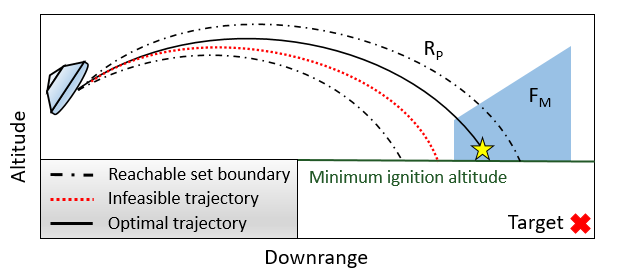
\includegraphics[width=0.8\textwidth]{../AAS20/Optimization} 
	\caption{The guidance algorithm seeks both the propellant-optimal ignition point (indicated by a star on the plot) and the trajectory whose optimal ignition point is best (indicated by the solid black line). The red, dotted trajectory is valid entry trajectory within the reachable set, but is infeasible because it does not intersect the powered descent feasible subset $\mathcal{F}_M$.}
	\label{fig_optimization}
\end{figure}

%At the core of the proposed entry phase guidance approach is an extension of the trajectory prediction to include the following powered descent phase. This allows one to alter the entry guidance objective from range control to propellant minimization. After applying several constraints to filter down the set of potential ignition states, the powered descent guidance is used to generate predictions of the propellant required from different states. The lowest among them is selected as the planned handoff condition from entry to powered descent. Further details on these constraints are given later.

%Notice that although propellant minimization is the entry guidance objective, any powered descent guidance algorithm with pinpoint landing capability may be used in the powered descent phase so long as an estimate of the propellant required is given by the algorithm, and this estimate is continuous with respect to the initial state. Thus, although in the examples of this work we have coordinated the powered descent phase to also be propellant-optimal in nature by solving the associated OCP, there exist many alternatives such as energy-optimal guidance or non-optimization based approaches such as polynomial guidance. 

%We further assume that the chosen powered descent method incorporates any necessary problem constraints, because the entry guidance algorithm does not make use of the predicted powered descent trajectory, nor does it check for satisfaction of constraints, but instead utilizes only the propellant cost associated with the powered descent trajectory. 
\subsection{Bank Angle Parametrization}
The entry phase guidance problem is intended to be solved onboard and so motivates a low-order parametrization of the bank angle profile. Parametrizing the bank angle function converts the optimal control problem into a more tractable nonlinear optimization problem. The choice of parametrization has important implications on the entry reachable set. The entry phase reachable set from an initial state $ \mathbf{x}_0$ is a tube of trajectories satisfying the equations of motion under admissible control functions 
\begin{equation*}
\mathcal{R}(\mathbf{x}_0)=\left\{\mathbf{x} \,| \,\exists\, t_f \;\mathrm{and}\; \sigma[0, t_f] \,\mathrm{with}\, \mathbf{x} = \varphi(t_f;\mathbf{x}_0,\, \sigma[0, t_f])  \right\}
\end{equation*}
and the portion of the reachable set that is of interest is its intersection with the powered descent feasible subset, i.e., $\mathcal{R} \cap \mathcal{F}_M$. Conceptually, by parametrizing the bank angle function in a particular way, we restrict the possible bank angle functions that can be generated, and as result will reduce the size of the reachable set. Let $R_P$ be the reachable set corresponding to a parametrization $ P $.
%The P-parametrized bank angle profile is a function of a finite set of parameters $P = \left\{p_1, p_2, ...,p_N \right\}$ and an associated function $h(\cdot)$ that defines the bank angle for each state, $\sigma(t) = h(P(x(t)))$.
%The dependence is to indicate closed loop nature, i.e. the values that P takes on change with the state unless flying perfectly along the optimal trajectory already 
%The P-parametrized reachable set is 
%\begin{equation*}
%\mathcal{R}(\mathbf{x}_0)=\left\{\mathbf{x} \,| \,\exists\, t_f \;\mathrm{and}\; \sigma(t)\,\forall\, t\in\,[0,t_f] \,\mathrm{with}\, \mathbf{x} = \varphi(\mathbf{x}_0; \sigma(t))  \right\}
%\end{equation*}
%$R_P(\mathbf{x}_0) =\left\{\mathbf{x}_f \,| \,\exists\, t_f \land\, P(\mathbf{x}) \,\mathrm{such\, that}\, \mathbf{x}_f = \varphi(t_f;\,\mathbf{x}_0,\, P(x(t))))  \right\} $. 
The relative size of $\mathcal{R}_P \subset \mathcal{R}$ is not the only consideration in choosing a parametrization. 
It is also desirable that $\mathcal{R}_P$ retains the propellant optimal point (or set) and neighboring region. 
%More formally, in addition to considering the effects of a parametrization on some measure of $\mathcal{R}_P\cap \mathcal{R}$, one may also consider the optimality gap, 
As a result, one might like to compare the propellant cost associated with a parametrization with the optimal solution over all parametrizations, i.e., compute
\begin{align}
\delta m = \left( \min_{x\in (\mathcal{R}\cap \mathcal{F}_M)} \mathrm{OCP}(x)\; - \min_{x\in (\mathcal{R}_P\cap \mathcal{F}_M)} \mathrm{OCP}(x) \right) \; \ge 0
\end{align}
in order to assess its quality, but this may be difficult to do. Instead, the minimum propellant costs of any two parametrizations can be compared against one another directly.  Let $\lambda$ be a measure of the volume of a state space set. Let $ P_A $ and  $ P_B $ be two different parametrizations, such that $\lambda(\mathcal{R}_{P_A}) < \lambda(\mathcal{R}_{P_B})$, and $\lambda(\mathcal{R}_{P_A}\cap \mathcal{R}) < \lambda(\mathcal{R}_{P_B}\cap \mathcal{R})$.
%but $\lambda(\mathcal{R}_{P_A}\cap \mathcal{F}_M) > \lambda(\mathcal{R}_{P_B}\cap \mathcal{F}_M)$.
Figure~\ref{fig_sets} depicts the relationship between the sets $\mathcal{F}_M,\,\mathcal{R},\,\mathcal{R}_{P_A},\,\mathrm{and}\,\mathcal{R}_{P_B}$ as well as a possible situation to demonstrate the possibility that $ \mathcal{R}_{P_A} $ is smaller than $\mathcal{R}_{P_B}$, and can reach less of $R$, yet has a smaller optimality gap than parametrization $ P_B $. 
\begin{figure}[h!]
	\centering
	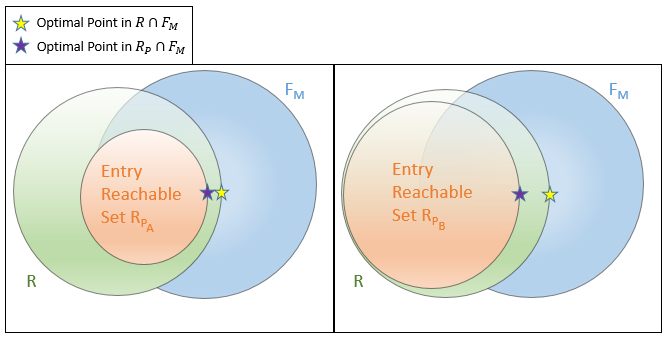
\includegraphics[width=0.9\textwidth]{../AAS20/SetDefinitions} 
	\caption{Consider two different parametrizations of the control, $ P_A $ and $ P_B $. While $ P_B $ allows the vehicle to reach more of the reachable set $\mathcal{R} $ than  $P_A$, much of $ R_{P_B}$ does not intersect $\mathcal{F}_M$. Additionally, the propellant optimal point in $ R_{P_A}$ is better than the optimal point in $ R_{P_B}$, indicated by the smaller distance between the optima, which are depicted with stars.  Note that these sets, depicted notionally as convex 2-D shapes, are actually 6-D and no claim is made about their convexity.}
	\label{fig_sets}
\end{figure}
%TODO: Better describe the stars? 
%Despite $ R_{P_B} $ being a larger set encompassing more of the true reachable set $R$, the intersection $R_{P_A}\cap \mathcal{F}_M$ is ``larger" than $R_{P_B}\cap \mathcal{F}_M$ and more importantly $ R_{P_A} $ encompasses a key subset of $ R $ – the region near the optimum. The difference between the two different optima is the sub-optimality gap imposed by the chosen parametrization.

The commanded bank angle profile considered here is a constant bank angle magnitude $\sigma_c$ with one bank reversal at a velocity $v_r$ and the current velocity $V$ is used as the independent variable in place of time,
\begin{equation}
\sigma(V; \sigma_c, \,v_r) = \left\{
\begin{array}{ll}
\sigma_c & V\geq v_r \\
-\sigma_c & V < v_r
\end{array} 
\right. .
\end{equation}
These commands are fed to a rate limiter to approximate the nature of a reaction control system tracking the commands. Because the profile includes a reversal, it offers a means to control lateral motion. 

The parametrization remains the same after the reversal, but the guidance continues to update the parameter values. By setting the lower bound on $v_r$ to be less than the ignition velocity during optimization, or greater than the current velocity, there exists the possibility to have one or no reversal planned at each update. This allows for as many reversals as there are optimization updates, but in simulations there will only be one or two reversals unless significant perturbations to the vehicle's planned heading occur after the first reversal. If an additional reversal is desired to eliminate large crossrange excursions, the parametrization is easily amended to accommodate one. A second reversal can be placed at a fixed velocity, and, exactly as the algorithm is currently applied, the first reversal timing is optimized until the reversal has been completed. Then, the second reversal is treated as the new optimization variable in addition to the bank angle magnitude. Such a ``one-at-a-time" strategy was put forth in Ref.~\cite{GuangfeiReplanning}. The result is, instead of one reversal with occasionally a second, all trajectories will feature two reversals with potential for a third. 

For comparison, we also consider a second parametrization of the form 
\begin{equation}
\sigma(V; \,v_1, \,v_2) = \left\{
\begin{array}{ll}
\;\;90^{\circ} & V\geq v_1 \\
-90^{\circ} & v_2 < V < v_1 \\
\;\;0^{\circ} & V \le v_2
\end{array} 
\right.
\end{equation}
where the two parameters $v_1,\, v_2$ such that $v_1 > v_2$ dictate the timing of the bank reversals, and the bank angle magnitudes are fixed.

\begin{figure}[h!]
		\centering
		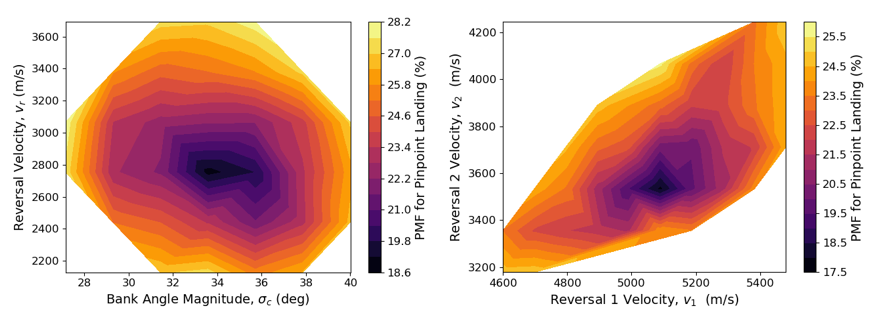
\includegraphics[width=1\textwidth]{../AAS20/ObjectiveContours} 
		\caption{Example contours of the propellant cost of pinpoint landing using two different parametrizations: a constant bank angle with one reversal, and a profile with two reversal velocities. Not only does the choice affect the propellant contours, but the reachable set is quite different as well. The downrange targeted in the constant profile is 700 km and is not reachable by the second parametrization, which instead targets 625 km. }
		\label{fig_objective_contour}
\end{figure}
%The entry guidance requires that the chosen powered descent guidance approach admits continuous propellant requirements for continuous ignition states to a fixed target. Atmospheric entry dynamics are smooth for smooth bank angle inputs and we thus expect that even when optimizing the ignition condition along a trajectory rather than use a fixed state variable such as velocity or energy, the objective function should be well-behaved and amenable to optimization. 
One key question when optimizing the parameters of the bank angle profile is whether there exist several isolated minima, or only a single global minimizer. 
Evaluating the objective function for a grid of the parameters defining the bank profile in each parametrization yields Figure~\ref{fig_objective_contour}, and indicates the objective function is likely convex, with steep gradients away from the optimum. From this, and repeated optimizations at various possible points, there is always a clear optimum.  The right plot of Figure~\ref{fig_objective_contour} shows that the two reversal parameters are significantly more coupled than the constant bank magnitude parametrization. This makes sense, as each reversal has a strong impact on the final heading, while in the constant bank parametrization, the bank magnitude has a much weaker affect on the heading than the reversal velocity. Clearly the choice of parametrization affects not only the shape of these contours, but also the minimum PMF achievable, as the second parametrization has a superior optimum. Note, however, that due to the difference in reachable set between the two parametrizations, the optimal downrange distance from the entry interface is different. For simplicity, the constant parametrization is adopted for the results in this paper. A more detailed analysis of the choice of parametrization is left for future work.

The shape of these objective functions indicates that gradient-based methods should be effective in determining the optimal profile parameters, however, determining the gradient of the objective function with respect to the switching velocity is generally difficult. As a result, derivative-free methods are preferred for this application. Powell's conjugate direction method \cite{PowellsMethod} is used in all of the examples herein. It is effective because for the chosen parametrization, the contours are nearly independent, so 1-D searches over each bounded parameter can very quickly locate the optimum. 

\subsection{Powered Descent Propellant Mapping}
By repeatedly solving the powered descent optimal control problem, Eq.~\ref{eq_srp_ocp}, for different ignition states, a pointwise approximation of a subset of the pinpoint landing feasible set $\mathcal{F}_M$ is computed via sampling. The full descent state vector is 7-D, but with two degenerate dimensions: the crossrange velocity, which is always zero by definition, and the initial mass, which is assumed to be fixed. A consequence of the dimensionality of the state space is a requirement to compute a large number of solutions -  16,807 solutions are required to span each of the remaining 5 dimensions with only 7 points. From sampled solutions we construct an approximation of the propellant costs for states in $\mathcal{F}_M$. Sampling is applicable irrespective of the powered descent algorithm to be used; for the problem of constrained propellant-optimal solutions, there exist significantly more efficient methods of computing the set $\mathcal{F}_M$ and the associated propellant cost, such as the convex optimization-based approach detailed in Ref.~\cite{SRP_ControllableSets}.

This mapping may be stored and interpolated in a variety of ways. Neural networks and other machine learning approaches were considered for their universal function approximation property. However, upon examination of the shape of the 5-D space together with numerical validation using additional OCP sample solutions, piecewise-linear 5-D interpolation was chosen to approximate the propellant mapping.
%The set of initial states over which to solve the OCP is computed by Latin Hypercube Sampling. After applying the constraints Eq~\ref{eq_constraints}, the OCP is solved for the remaining states. The model is constructed 
%TODO: Note (as Mease mentioned) that because the table is defined in SRP coordinates, it implicitly exploits the rotational symmetry as well 
%TODO: Iterative scheme
%TODO: Note the approximation is enabling, allowing MANY srp problems to be "solved" onboard
%, allowing the use of 5-D interpolation rather than 6-D. The absolute value of the crossrange distance is used because this gives a denser table of tabulated solutions by exploiting symmetry resulting from the zero crossrange velocity. 

\subsection{Trajectory Prediction and Powered Descent Ignition}
Once the bank angle parametrization is specified, the estimated entry state is integrated numerically to generate a prediction of the remaining unpowered entry trajectory. The components of the constraint vector Eq.~\ref{eq_constraints} used in the definition of $\mathcal{F}_M$ are then applied to the predicted trajectory to determine the interval that should be checked for the propellant-optimal transition to powered descent. These constraints greatly reduce the number of calls to the descent guidance propellant mapping required to find the optimum. As a reminder, these constraints include an upper bound on velocity corresponding to the maximum achievable deceleration with the available propellant, a minimum ignition altitude required for safe powered descent and subsequent EDL operations, and a maximum distance to the target, again related to the available propellant. Figure~\ref{fig_ignition} depicts this process including a portion of the trajectory already flown, the entry flight prediction, constraints, pinpoint landing target, and predicted optimal ignition point. 

Once the constraints have been applied, 1-D optimization is applied to the remaining trajectory interval, indicated by the dash black line, by viewing the fixed trajectory as a function of some independent variable. Our implementation uses velocity as the independent variable over which to search, but time or distance are also possibilities. 1-D optimization is used to very quickly locate the optimum, rather than determine the solution by brute force by checking all of the remaining points. Once the solution is determined, the commanded bank angle sign and magnitude are computed as a function of the vehicle estimated velocity, and are then sent to the control system.
%The numerical integration of the entry state is carried out using downrange distance to the target as the independent variable. Using range to go as the independent variable allows the terminal integration condition to be zero, independent of the problem specifics, with very little wasted integration time since the optimal ignition state is generally close to the target. 
%This has several advantages over common alternatives. First, although energy or velocity could be used, a sufficiently low choice of the terminal value must be made, but any time spent integrating below the reachable set of the vehicle is wasted, and the choice is problem/vehicle specific. Altitude would also be a natural choice since the minimum ignition altitude would serve as the terminal integration condition, but like energy and velocity this is problem-dependent, and additionally altitude is not a strictly monotonic variable in the case of lofting trajectories.
\begin{figure}[h!]
	\centering
	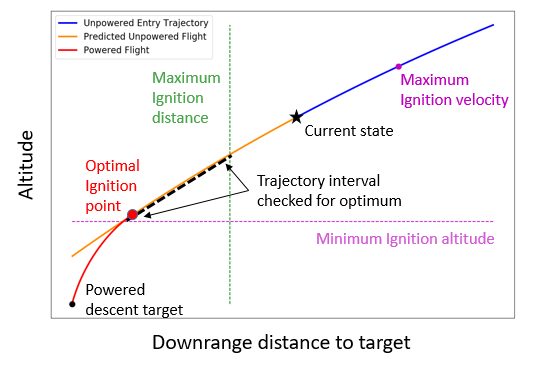
\includegraphics[width=0.7\textwidth]{../AAS20/H_Vs_S} 
	\caption{Only the interval of the predicted entry trajectory satisfying constraints on velocity, altitude, and distance to the target are searched for the propellant-optimal ignition state.}
	\label{fig_ignition}
\end{figure}


%%% Local Variables: ***
%%% mode: latex ***
%%% TeX-master: "thesis.tex" ***
%%% End: ***
